\section{Efficient Attention}

\begin{frame}{}
    \LARGE Next-Generation Architectures: \textbf{Efficient Attention}

    \vspace{1em}
    \normalsize Can we keep attention, and its exact recall, but pay less for it?
\end{frame}

\begin{frame}{Four Ways to Pay Less for Attention}
    \begin{center}
    \small
    \renewcommand{\arraystretch}{1.3}
    \begin{adjustbox}{max width=\linewidth}\begin{tabular}{>{\raggedright\arraybackslash}p{3.6cm}>{\raggedright\arraybackslash}p{5.0cm}>{\raggedright\arraybackslash}p{4.4cm}}
        \toprule
        \textbf{Idea} & \textbf{What it changes} & \textbf{Still exact attention?} \\
        \midrule
        Better kernels & how the same maths runs on the GPU & yes \\
        Local windows & each token sees only its neighbours & no, long range is cut \\
        Learned sparsity & each token sees a \emph{chosen} subset & no, but the model picks \\
        Context parallelism & one sequence is split across GPUs & yes \\
        \bottomrule
    \end{tabular}\end{adjustbox}
    \end{center}
    \vspace{0.3em}
    \begin{itemize}\itemsep0.5em
        \item The first idea dates from 2022. \textbf{FlashAttention} computes exact attention in tiles that fit in fast on-chip memory, and never writes the $L\times L$ matrix out.
        \item That fixed the bottleneck of its day, which was \emph{memory traffic}. The hardware then moved on. So did the bottleneck.
    \end{itemize}
\end{frame}

\subsection{Faster Kernels: FlashAttention-3 and 4}

\begin{frame}{FlashAttention-3: When Softmax Became the Slow Part}
    \begin{itemize}\itemsep0.4em
        \item On an H100, matrix multiply runs at \textbf{989 TFLOPS}. Special functions such as $\exp$ run at \textbf{3.9}. FlashAttention-2 reaches only about 35\% of the GPU's peak.
        \item \textbf{Idea 1, overlap.} Two groups of threads take turns: while one does the softmax, the other runs matrix multiplies. The slow step hides under the fast one.
    \end{itemize}
    \centering
    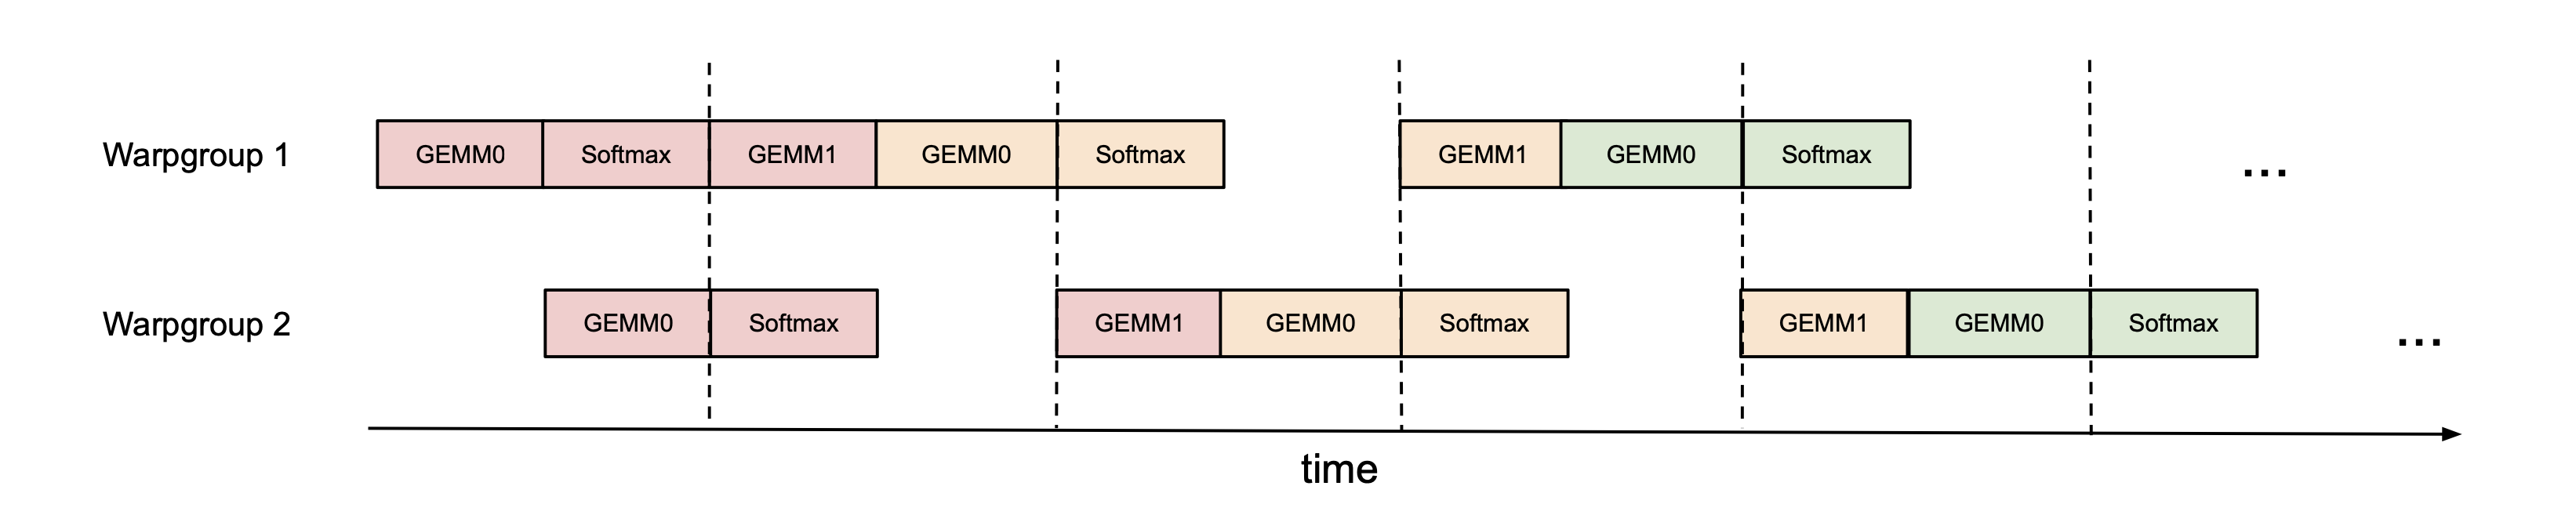
\includegraphics[width=0.82\linewidth,height=0.24\textheight,keepaspectratio]{images/next-gen-architectures/fa3_fig1_pingpong.png}
    \begin{itemize}\itemsep0.4em
        \item \textbf{Idea 2, FP8.} Halve the precision, double the throughput. Per-block scaling and a random rotation of $Q$ and $K$ keep the error 2.6$\times$ below naive FP8.
        \item \textbf{Result:} 1.5 to 2$\times$ faster than FlashAttention-2, up to 740 TFLOPS (75\% of peak).
    \end{itemize}
    \src{Shah et al., ``FlashAttention-3: Fast and Accurate Attention with Asynchrony and Low-precision,'' \href{https://arxiv.org/abs/2407.08608}{arXiv:2407.08608}, Figure 1 and Table 3. Dao, FlashAttention-3 blog (2024).}
\end{frame}

\begin{frame}{FlashAttention-4 (2026): Hardware Scales Unevenly}
    \begin{itemize}\itemsep0.5em
        \item From H100 to B200, tensor-core throughput grew about \textbf{2.25$\times$}. The units that compute $\exp$, and shared-memory bandwidth, \textbf{did not grow}.
        \item So the exponential is now a co-bottleneck in the forward pass. FlashAttention-4 answers with algorithm changes, not only scheduling:
        \begin{itemize}\itemsep0.25em
            \item compute part of the $\exp$ calls in \emph{software}, with a cubic polynomial on idle arithmetic units
            \item rescale the running softmax only when the maximum jumps
            \item keep intermediate tiles in the new on-chip tensor memory
        \end{itemize}
        \item \textbf{Result:} 1613 TFLOPS on a B200 (71\% of peak), up to 1.3$\times$ over cuDNN.
    \end{itemize}
    \vspace{0.2em}
    \takeaway{Each GPU generation moves the binding resource: memory traffic, then thread scheduling, then $\exp$ throughput. A kernel is never finished.}
    \src{Zadouri et al., ``FlashAttention-4: Algorithm and Kernel Pipelining Co-Design for Asymmetric Hardware Scaling,'' \href{https://arxiv.org/abs/2603.05451}{arXiv:2603.05451}. Dao, FlashAttention-4 blog (2026).}
\end{frame}

\subsection{Sliding-Window Attention}

\begin{frame}{Sliding-Window Attention in Production}
    \begin{itemize}\itemsep0.3em
        \item Kernels do not shrink the KV cache. The simplest way to do that: \textbf{most layers look only at recent tokens}.
    \end{itemize}
    \begin{center}
    \small
    \renewcommand{\arraystretch}{1.15}
    \begin{adjustbox}{max width=\linewidth}\begin{tabular}{lll}
        \toprule
        \textbf{Model} & \textbf{Pattern (local : global layers)} & \textbf{Window} \\
        \midrule
        Mistral 7B (2023) & all local & 4096 \\
        Gemma 2 (2024) & 1 : 1 & 4096 \\
        Gemma 3 (2025) & 5 : 1 & 1024 \\
        gpt-oss (2025) & 1 : 1, with learned attention sinks & 128 \\
        Llama 4 (2025) & 3 : 1, local layers attend within fixed chunks & 8192 \\
        \bottomrule
    \end{tabular}\end{adjustbox}
    \end{center}
    \begin{itemize}\itemsep0.3em
        \item The trend: \textbf{windows shrink, and a few global layers carry the long range}.
        \item Gemma 3: KV memory overhead at 32K tokens falls from about 60\% to under 15\%.
        \item The same shape as the hybrids. Cheap layers do most of the work, and a few expensive ones keep the capability.
    \end{itemize}
    \src{Jiang et al., \href{https://arxiv.org/abs/2310.06825}{arXiv:2310.06825}. Gemma Team, \href{https://arxiv.org/abs/2408.00118}{arXiv:2408.00118} and \href{https://arxiv.org/abs/2503.19786}{arXiv:2503.19786}, Figure 5. OpenAI, \href{https://arxiv.org/abs/2508.10925}{arXiv:2508.10925}. Hugging Face, Llama 4 release blog (2025).}
\end{frame}

\begin{frame}{What a Window Cannot See}
    \begin{itemize}\itemsep0.55em
        \item \textbf{A common misreading.} Stacking $k$ layers of window $W$ gives a theoretical span of $W\times k$. That is a receptive field, not reliable long-range recall.
        \item \textbf{Evidence.} In MiniMax's ablation, full attention scores 90 on RULER at 128K. The sliding-window variant scores 72.
        \item \textbf{Memory is not latency.} Mistral dropped sliding windows in a later model: they reduce memory but do not necessarily reduce inference latency.
        \item Fixed patterns were tried long ago (Sparse Transformer, Longformer, BigBird, 2019 to 2020). Only the local window survived.
    \end{itemize}
    \vspace{0.3em}
    \takeaway{A fixed pattern decides where to look before reading the input. What if the model \emph{chose} which distant tokens matter?}
    \src{Raschka, ``MiniMax M2 Technical Report Notes'' (May 2026) and ``The Big LLM Architecture Comparison'' (2025, updated 2026). Child et al., \href{https://arxiv.org/abs/1904.10509}{arXiv:1904.10509}. Beltagy et al., \href{https://arxiv.org/abs/2004.05150}{arXiv:2004.05150}. Zaheer et al., \href{https://arxiv.org/abs/2007.14062}{arXiv:2007.14062}.}
\end{frame}

\subsection{Learned Sparse Attention}

\begin{frame}{Native Sparse Attention: Three Views of the Past}
    \centering
    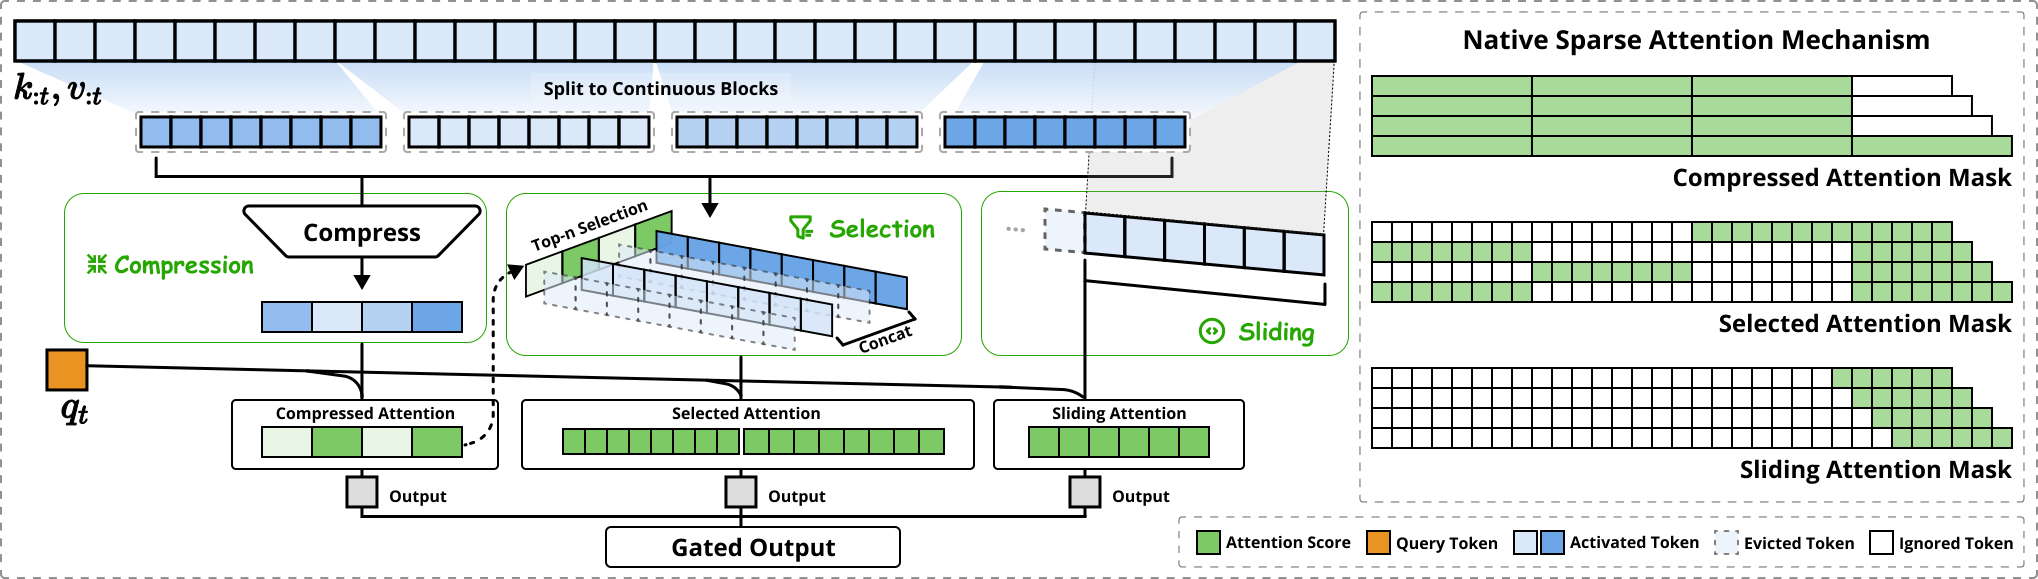
\includegraphics[width=0.95\linewidth,height=0.4\textheight,keepaspectratio]{images/next-gen-architectures/nsa_fig2_architecture.png}
    \begin{itemize}\itemsep0.35em
        \item Each query attends through three branches, mixed by learned gates:
        \textbf{compressed} blocks (a coarse view of everything), \textbf{selected} blocks (the top-$n$ most relevant, at full detail), and a \textbf{sliding window}.
        \item The compressed scores are reused to choose the blocks, so selection is almost free.
        \item Trained sparse from the start. At 64K context: 11.6$\times$ faster decoding and 9$\times$ faster forward pass, with benchmark scores at or above the full-attention baseline.
    \end{itemize}
    \src{Yuan et al., ``Native Sparse Attention: Hardware-Aligned and Natively Trainable Sparse Attention,'' \href{https://arxiv.org/abs/2502.11089}{arXiv:2502.11089}, Figure 2. Reported by the authors and not yet independently replicated.}
\end{frame}

\begin{frame}{DeepSeek Sparse Attention: A Cheap Scorer Picks 2048 Tokens}
    \begin{itemize}\itemsep0.45em
        \item A tiny \textbf{lightning indexer} scores every past token for the current query:
        \[
            I_{t,s}=\sum_{j=1}^{H^I} w^I_{t,j}\;\mathrm{ReLU}\big(q^I_{t,j}\cdot k^I_s\big)
        \]
        \item Only the \textbf{top 2048} tokens go to the real attention. Its cost falls from $O(L^2)$ to $O(Lk)$.
        \item \textbf{It can be retrofitted.} DeepSeek converted a dense checkpoint: a short warm-up where the indexer imitates dense attention, then sparse training. GLM-5 repeated the recipe with only 20B tokens.
        \item \textbf{Impact:} DeepSeek cut API prices by more than 50\% with V3.2.
    \end{itemize}
    \vspace{0.1em}
    \takeaway{Contrast with Part 1. Hybrids \emph{compress} the past into a state. Sparse attention keeps every token and \emph{retrieves}.}
    \src{DeepSeek-AI, ``DeepSeek-V3.2,'' \href{https://arxiv.org/abs/2512.02556}{arXiv:2512.02556}. DeepSeek API news (Sep 2025). Zhipu AI, ``GLM-5,'' \href{https://arxiv.org/abs/2602.15763}{arXiv:2602.15763}.}
\end{frame}

\begin{frame}{DeepSeek-V4: Compress First, Then Select}
    \begin{columns}[T,onlytextwidth]
        \column{0.6\textwidth}
        \begin{itemize}\itemsep0.45em
            \item One problem remained: the indexer still scans every token. V4 shrinks the sequence \emph{before} scoring.
            \item Two layer types alternate through the network:
            \begin{itemize}\itemsep0.25em
                \item \textbf{CSA}: compress keys and values 4$\times$, then keep the top-$k$ compressed entries. A sparse, fine view.
                \item \textbf{HCA}: compress 128$\times$ and attend to all of it. A dense, coarse view.
            \end{itemize}
            \item Every layer adds a window of 128 recent uncompressed tokens.
            \item At 1M tokens, a CSA layer in V4-Pro reads about 1,150 entries. An HCA layer reads about 8,300.
        \end{itemize}
        \column{0.38\textwidth}
        \centering
        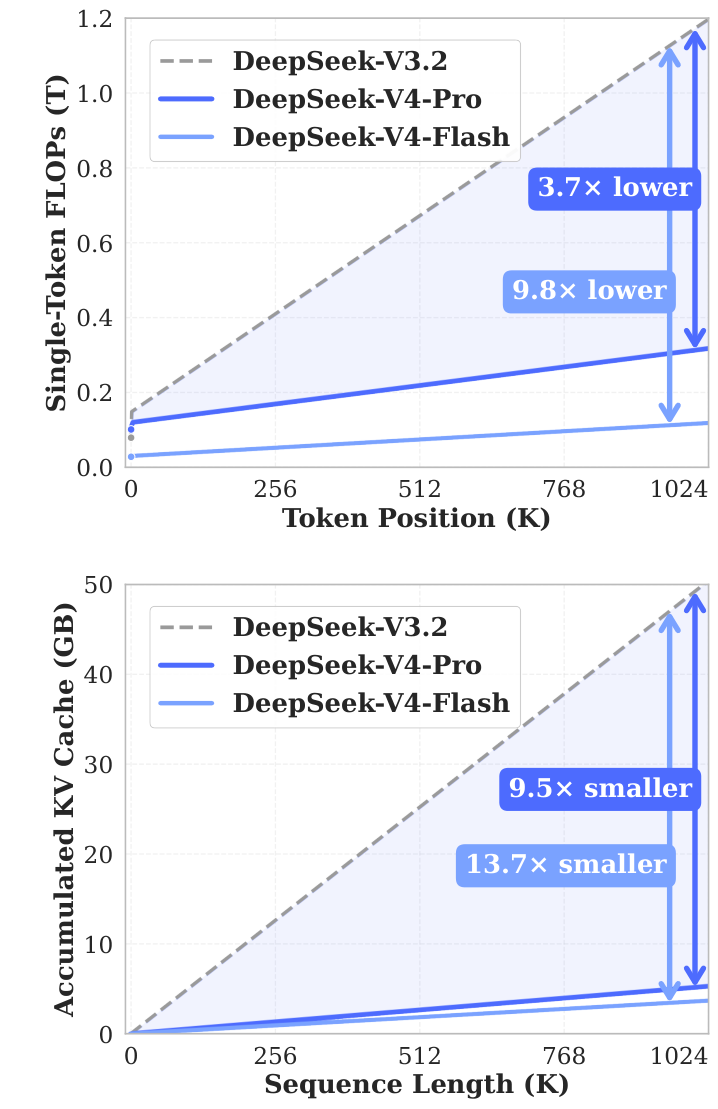
\includegraphics[width=\linewidth,height=0.62\textheight,keepaspectratio]{images/next-gen-architectures/dsv4_fig1_right_flops_kv.png}
    \end{columns}
    \vspace{0.2em}
    \src{DeepSeek-AI, ``DeepSeek-V4,'' \href{https://arxiv.org/abs/2606.19348}{arXiv:2606.19348}, Figure 1 (right) and Section 2.3. Entry counts derived from the published hyperparameters ($k=1024$, window 128, $2^{20}/128$).}
\end{frame}

\begin{frame}{Is Sparse Attention Ready? A Seven-Month Reversal}
    \begin{itemize}\itemsep0.55em
        \item \textbf{November 2025.} MiniMax ships M2 with full attention and writes that no efficient variant has shown stable superiority in production.
        \item \textbf{June 2026.} MiniMax ships M3 with its own block-sparse attention: 14.2$\times$ faster prefill and 7.6$\times$ faster decoding at 1M tokens, on par with the dense baseline.
        \item \textbf{What changed?} Not the idea. The \emph{kernels} (selection matched to GPU blocks) and the \emph{training recipes} (adapt from a dense checkpoint).
        \item The frontier in mid-2026 is the indexer itself. GLM-5.2 reuses one indexer result across four layers and removes 75\% of the indexer's compute.
        \item No training budget? \textbf{Training-free} methods (Quest, MInference, DuoAttention) select KV entries at inference time on an unmodified model.
    \end{itemize}
    \src{MiniMax, ``No Free Lunch'' blog (LMSYS, Nov 2025). Lai et al., \href{https://arxiv.org/abs/2606.13392}{arXiv:2606.13392}. Bai et al., ``IndexCache,'' \href{https://arxiv.org/abs/2603.12201}{arXiv:2603.12201}. Tang et al., \href{https://arxiv.org/abs/2406.10774}{arXiv:2406.10774}.}
\end{frame}

\subsection{Ring Attention and Context Parallelism}

\begin{frame}{Ring Attention: One Sequence, Many GPUs}
    \begin{columns}[T,onlytextwidth]
        \column{0.56\textwidth}
        \begin{itemize}\itemsep0.45em
            \item Everything so far saves compute on \emph{one} device. Training on million-token sequences needs the opposite: \textbf{split one sequence across devices}.
            \item Each device keeps its own block of queries. Key and value blocks \textbf{travel around a ring}.
            \item FlashAttention's blockwise softmax makes the order of arrival irrelevant, so the result is exact.
            \item Sending a block overlaps with computing on the previous one. Communication is free if each block is large enough: about 1,000 tokens on an A100.
            \item Memory per device no longer depends on total sequence length.
        \end{itemize}
        \column{0.42\textwidth}
        \centering
        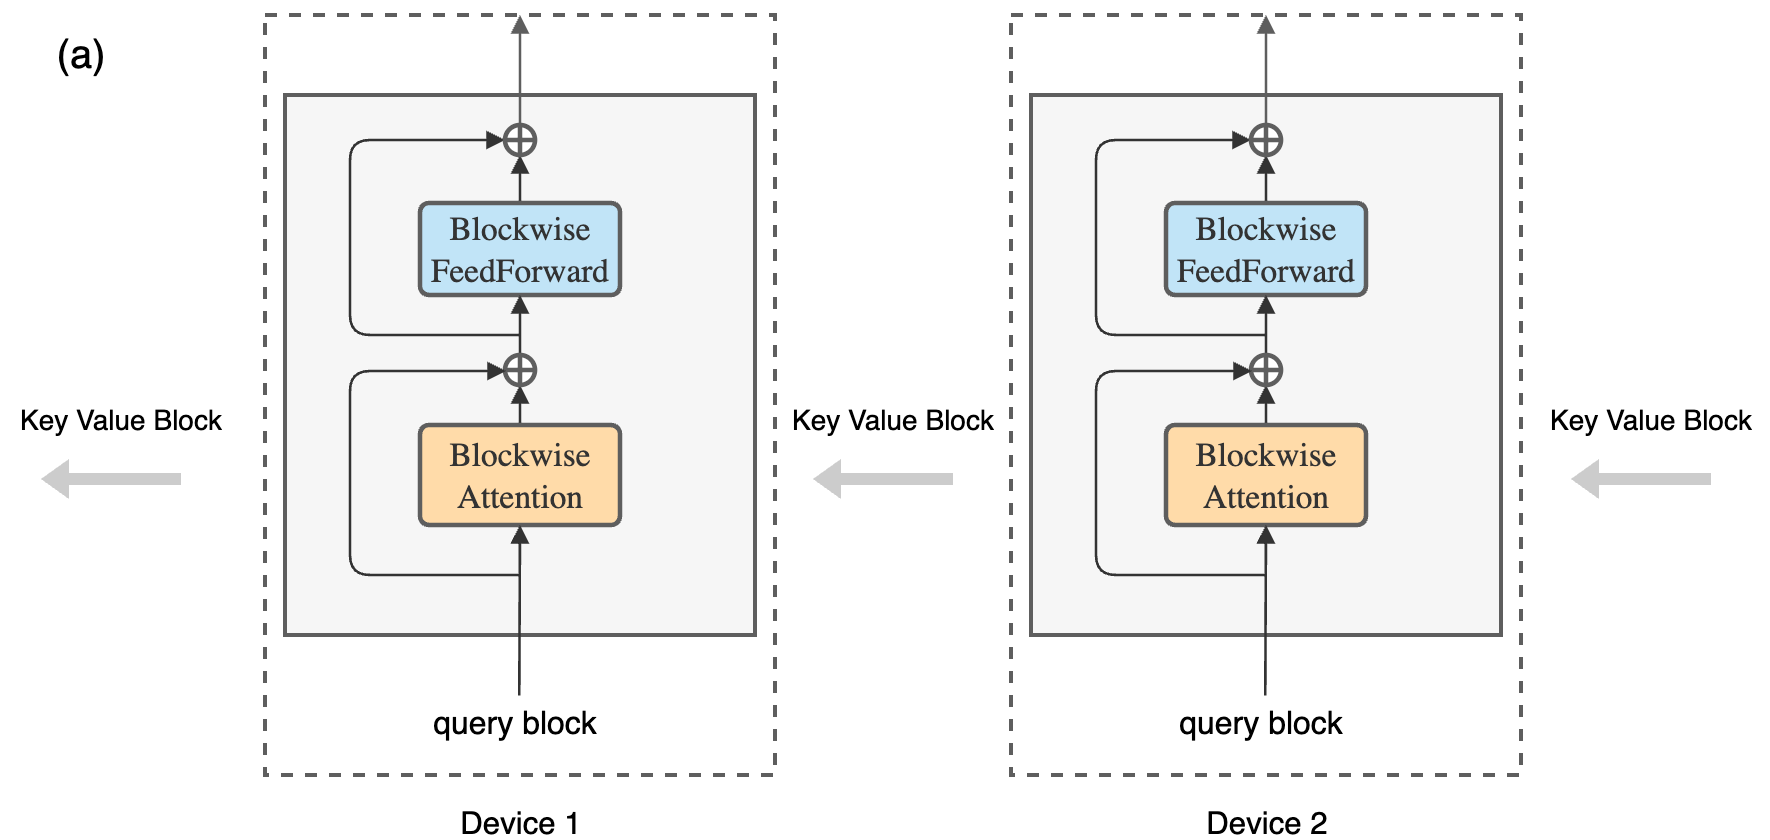
\includegraphics[width=\linewidth,height=0.6\textheight,keepaspectratio]{images/next-gen-architectures/ring_attention_fig2a_kv_blocks_traverse_ring.png}
    \end{columns}
    \src{Liu, Zaharia, Abbeel, ``Ring Attention with Blockwise Transformers for Near-Infinite Context,'' \href{https://arxiv.org/abs/2310.01889}{arXiv:2310.01889}, Figure 2.}
\end{frame}

\begin{frame}{Context Parallelism in Practice}
    \begin{itemize}\itemsep0.5em
        \item \textbf{Problem with a plain ring under a causal mask:} the device holding the last tokens has far more work than the one holding the first. \emph{Striped Attention} interleaves tokens across devices to even the load.
        \item \textbf{What Meta did for Llama 3.} No ring at all. Each device simply gathers all keys and values. Two reasons: with grouped-query attention the KV tensors are small, and the gather is $O(S)$ under an $O(S^2)$ computation.
    \end{itemize}
    \begin{center}
    \small
    \begin{adjustbox}{max width=\linewidth}\begin{tabular}{llc}
        \toprule
        \textbf{Setup} & \textbf{Sequence length} & \textbf{GPU utilisation (MFU)} \\
        \midrule
        Llama 3, 16,384 GPUs, 16-way context parallel & 131,072 & 38\% \\
        torchtitan, Llama3-8B on 32 H100, all-gather & 1M & 25.7\% \\
        torchtitan, same, ring-style all-to-all & 1M & 12.1\% \\
        \bottomrule
    \end{tabular}\end{adjustbox}
    \end{center}
    \begin{itemize}
        \item \textbf{Open question:} how to split learned sparse attention, where the tokens a query needs are not known in advance.
    \end{itemize}
    \src{Brandon et al., \href{https://arxiv.org/abs/2311.09431}{arXiv:2311.09431}. Meta, ``The Llama 3 Herd of Models,'' \href{https://arxiv.org/abs/2407.21783}{arXiv:2407.21783}, Table 4. PyTorch forum, ``Training long-context LLMs with 1M sequence length using context parallel'' (Jan 2025).}
\end{frame}

\begin{frame}{Efficient Attention: What to Remember}
    \begin{itemize}\itemsep0.6em
        \item \textbf{Kernels} (FlashAttention-3 and 4) give exact attention at 70 to 75\% of GPU peak. They follow the hardware, generation by generation.
        \item \textbf{Windows} cut the KV cache cheaply, but a few global layers must remain.
        \item \textbf{Learned sparse attention} became a production default within 2025 to 2026: a cheap scorer, a top-$k$ selection, and a local window.
        \item \textbf{Context parallelism} is how million-token sequences are trained at all.
    \end{itemize}
    \vspace{0.4em}
    \takeaway{\textbf{Next.} We can now afford a million tokens. Affording them and \emph{using} them are different problems.}
\end{frame}
